\chapter{Platforma Android}

\section{Początki systemu}
Początki systemu Android sięgają roku 2003, kiedy to Andy Rubin, Chris White, Nick Sears oraz Rich Miner założyli w~Kalifornii firmę Android Inc. Głównym celem powstania przedsiębiorstwa była chęć produkcji urządzeń mobilnych, które bazowałyby na danych lokalizacyjnych i~uwzględniały preferencje użytkowników. Jednak zmagająca się z~wymaganiami rynku oraz trudnościami finansowymi firma w~2005 roku została przejęta przez Google Inc., amerykańskie przedsiębiorstwo z~branży internetowej, słynące z~popularnej wyszukiwarki o~tej samej nazwie. Wkrótce potem założono grupę \textit{Open Handset Alliance} (OHA), w~której skład weszły, oprócz Google, takie znane firmy jak HTC, Intel, Motorola, Qualcomm, T-Mobile, Sprint Nextel oraz NVIDIA, a~która stawiała sobie za cel rozwój otwartych standardów dla telefonii mobilnej. Zdecydowanie przyspieszyło to badania nad systemem i~jego rozwój. Pierwsza wersja Androida została przedstawiona światu już w~2007 roku, a~pierwszym telefonem, który korzystał z~tego systemu, był HTC G1.

Android nazywa kolejne wersje swoich systemów zgodnie z nazwami słodyczy. Dwa premierowe wydania nie miały kryptonimów. Dopiero wersja 1.5, która została wydana 30 kwietnia 2009 roku, otrzymała nazwę \textit{Cupcake}. Najnowsza wersja 6.0 posiada nazwę \textit{Marshmallow}, a~w~marcu 2016 ukazało się wydanie \textit{beta} systemu Android "N". Oficjalny kryptonim nie jest jeszcze znany.

\section{Udział w~rynku}
Android to system operacyjny przeznaczony przede wszystkim dla urządzeń mobilnych. Według \cite{website:android:stat2}, we~wrześniu 2015 roku miał on największy udział w~rynku tych urządzeń na~świecie, a~jego udział przekroczył 53\%. Jest to przedstawione na rysunku \ref{fig:android_udzial_zagranica}. Drugie miejsce na świecie według tego samego portalu zajmuje system iOS (38\%), a~trzecie - Windows Phone z~niespełna 3\% udziału. 

\newpage
\begin{figure}[!htb]
    \centering
    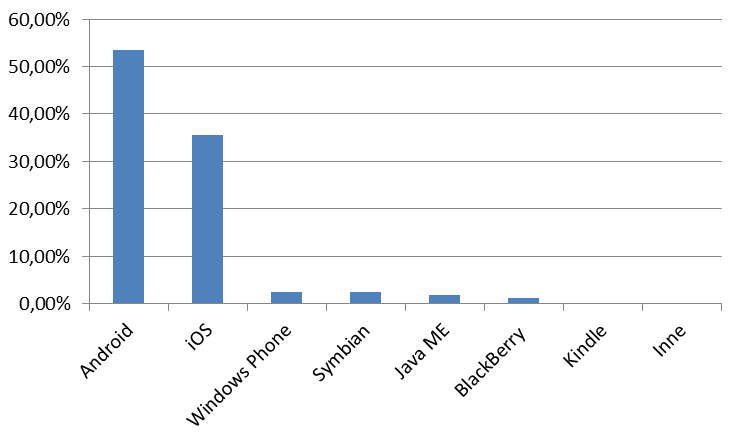
\includegraphics[width=12cm]{imgs/ch2_android_udzial_2pl.png}
    \caption
{Android – udział w~rynku urządzeń mobilnych na świecie\cite{website:android:stat2}.}
    \label{fig:android_udzial_zagranica}
\end{figure} 

W Polsce proporcje są nieco inne. Według \cite{website:android:stat1}, udział Androida na rynku urządzeń mobilnych wynosi 63.8\%. Na~drugim miejscu plasuje się system Windows Phone (15.7\%), a~trzeci iOS zajmuje tylko 10\%~rynku urządzeń mobilnych (rysunek \ref{fig:android_udzial_polska}).

\begin{figure}[!htb]
    \centering
    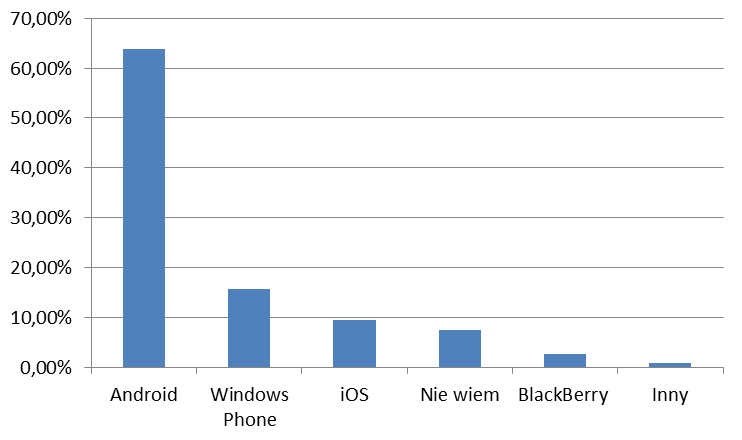
\includegraphics[width=12cm]{imgs/ch2_android_udzial_1pl.png}
    \caption
{Android – udział w~rynku urządzeń mobilnych w~Polsce \cite{website:android:stat1}.}
    \label{fig:android_udzial_polska}
\end{figure} 

\newpage

\section{Rozwój systemu}
Niezwykle cenną z~punktu widzenia programistów jest informacja o~udziale poszczególnych wersji Android na urządzeniach posiadanych przez użytkowników. Dzięki niej mogą oni lepiej zoptymalizować swoje aplikacje pod kątem sprzętu, na którym są uruchamiane. Według  \cite{website:android:spidersweb}, dane z~lutego 2016 przedstawiają się jak na rysunku \ref{fig:android_udzial_wersje}.

\begin{figure}[!htb]
    \centering
    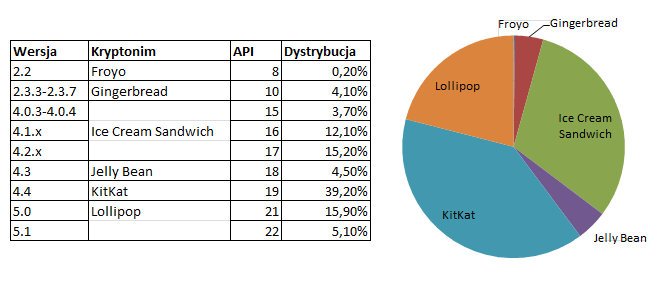
\includegraphics[width=16cm]{imgs/ch2_android_udzial_3pl.png}
    \caption
{Statystyki dotyczące używania poszczególnych wersji systemu Android przez użytkowników \cite{website:android:spidersweb}.}
    \label{fig:android_udzial_wersje}
\end{figure} 

Z urządzeń, na których instalowany jest Android, większość stanowią smartfony i~tablety. Również urządzenia takie jak \textit{smart-watches}, \textit{smart-TVs}, akcesoria telewizyjne, konsole do gier, piekarniki, pralki, lodówki, satelity wysyłane w~kosmos, a~także najnowsze dziecko firmy Google - Google Glass, wspomagane są tym popularnym systemem operacyjnym. Co więcej, firmy motoryzacyjne zaczynają instalować Androida w~\textit{head unitach} swoich samochodów, rozbudowując w~ten sposób platformę informacyjną i~rozrywkową.

Zgodnie z~manifestem założonej przez Google w~2007 roku grupy \textit{Open Handset Alliance} (OHA), Android został zbudowany z~wykorzystaniem wielu różnych komponentów na licencji \textit{Open Source}. Zalicza się do nich przede wszystkim jądro Linux, biblioteki programistyczne, kompletne interfejsy użytkownika, aplikacje i~wiele wiele innych. Większość kodu systemu Android jest wydana na licencji \textit{Apache Software License} (ASL, v 2.0). Wyjątkiem jest jądro Linuxa, które wykorzystuje GPLv2 oraz projekt \textit{WebKit} korzystający z~licencji BSD. 

Nie wszystkie części kodu Androida są otwarte dla programistów. Nawet urządzenia z~należącej do Google linii Nexus zawierają komercyjne sterowniki, algorytmy szyfrujące, a~nawet całe aplikacje. Jest to duże utrudnienie dla osób próbujących wykorzystać je do pisania własnych programów. Mimo tych utrudnień wielu programistów, nie pracując dla Google bezpośrednio, zaangażowanych jest w~tworzenie kodu nowych wersji systemu Android. W rozwijanie systemu są zaangażowani jednak nie tylko programiści. Wokół Androida zrzeszeni są również producenci procesorów, pamięci RAM, urządzeń, ekranów i~wielu innych części składających się na gotowy produkt.

\section{Programowanie w~systemie w~Android}
Jako system operacyjny dostępny na licencji \textit{Open Source}, Android zrzesza również ogromną społeczność programistów piszących aplikacje poszerzające funkcjonalność urządzeń. Najpopularniejszymi językami programowania, które wykorzystuje się do pisania aplikacji na Androida, są Java i~C++ ze środowiskiem \textit{Android NDK (Native Development Kit)}. 

Pisząc aplikacje dla Androida w~języku Java, programiści wykorzystują Android SDK (Software Development Kit). Ten zestaw narzędzi programistycznych składa się z~dwóch części: SDK Tools – wymaganej do pisania aplikacji niezależnie od wersji Androida, oraz Platform Tools – czyli narzędzi zmodyfikowanych pod kątem konkretnych wersji systemu. W~skład środowiska programistycznego wchodzi dokumentacja, przykładowe programy, biblioteki, emulator oparty na QEMU\footnote{QEMU - szybki emulator napisany przez Fabrice Bellarda.} oraz debugger. SDK dostępne jest zarówno dla Windowsa, Linuksa jak i~dla MacOSX.

Android SDK ma budowę modularną. Modułami są np. obrazy konkretnych wersji Androida, dodatkowe sterowniki, źródła SDK, czy przykładowe programy. Pomocne mogą być również obrazy systemu uruchamiane na emulatorze, dzięki którym programiści mogą  testować zachowanie aplikacji na różnych wersjach systemu Android, bez użycia fizycznych urządzeń \cite{website:wikipedia}.

Dużym ułatwieniem dla programistów Javy jest także Android Studio - zintegrowane środowisko programistyczne oparte na IntelliJ IDEA\footnote{IntelliJ IDEA – komercyjne zintegrowane środowisko programistyczne (IDE) dla Javy firmy JetBrains.}. Jego główne zalety to zarządzanie wieloma projektami, możliwość konfiguracji budowy programu w~kilku wariantach dla jednego projektu, możliwość automatycznego uzupełniania kodu oraz wykonywania testów jednostkowych i~integracyjnych bezpośrednio z~narzędzia.

Jako narzędzie służące do budowania projektów w~Javie wykorzystywany jest \textit{Gradle}. W~przeciwieństwie do jego poprzedników: \textit{Ant}-a i~\textit{Maven}-a, działa w~oparciu o~regułę \textit{„convention over configuration”} polegającą na zminimalizowaniu potrzebnej konfiguracji, poprzez używanie gotowych wartości domyślnych: jeżeli czegoś nie ma w~skrypcie konfiguracyjnym nie znaczy, że nie zostało skonfigurowane i~nie zostanie wykorzystane. Oznacza to tylko, że nie zostały zmienione wartości domyślne.

O~ile język Java wydawać się może najrozsądniejszym wyborem, o~tyle wielu programistów używa środowiska NDK. Jest to zestaw narzędzi, który pozwala realizować części aplikacji za pomocą kodu w~językach programowania~C~i~C++. Zazwyczaj środowisko to wykorzystuje się w~celu pisania programów, które intensywnie wykorzystują procesor, takich jak silniki gier, przetwarzania sygnału czy symulacji fizyki. Wykorzystywane jest również w przypadkach, gdy istnieje potrzeba napisania wspólnej biblioteki, która może zostać wykorzystana przez inne systemy operacyjne, takie jak iOS lub Windows Phone, lub wspólnej części zawierającej logikę biznesową wykorzystywaną przez różne aplikacje z różnych systemów operacyjnych. Jednak programiści muszą wziąć pod uwagę również wady takiego rozwiązania, które mogą nie do końca zbilansować korzyści. Natywny kod Androida na ogół nie powoduje zauważalnej poprawy wydajności \cite{website:java:wydajnosc}, zwiększa za to znacznie złożoność aplikacji. Podsumowując, z~NDK należy korzystać tylko wtedy, jeśli jest to niezbędne dla wytwarzanego programu. Zanim programista zdecyduje się na to rozwiązanie, najpierw powinien sprawdzić, czy środowisko programistyczne Androida nie zapewnia już funkcjonalności, jakiej potrzebuje.
%androidowe \textit{API\footnote{Interfejs programistyczny aplikacji (ang. Application Programming Interface, API) – sposób, rozumiany jako ściśle określony zestaw reguł i ich opisów, w jaki programy komputerowe komunikują się między sobą. \\textit{Application Programming Interface, Wikipedia, 2016}}} 

Java i~C czy C++ to jednak nie wszystkie języki, których można użyć przy programowaniu aplikacji na Androida. Podczas szukania materiałów do tej pracy autor spotkał się z~przykładami aplikacji napisanych w~C\#, Delphi, czy nawet w~języku Kotlin. Ten statycznie typowany język programowania działający na maszynie wirtualnej Javy jest zaprojektowany z~myślą o~pełnej interoperacyjności z~Javą i~polega na jej bibliotekach \cite{website:wikipedia}. %Języki te stanowią jednak tak mały udział, że nie będą one brane pod uwagę podczas analizy opisywanego problemu testowalności oprogramowania na ten system operacyjny.


%tutaj przykłady jak użyć poszczególnych konstrukcji
%Przykładowy rysunek \ref{fig:sample_figure}. Prztykładowa tabela %\ref{tab:sample_table}. Przykładowy odnośnik do bibliografi \cite{bib:kowalski_2015}. \textbf{Powodzenia!}


%\begin{figure}[!htb]
%    \centering
%    \includegraphics[width=10cm]{imgs/sample_figure.jpg}
%    \caption{Przykłady rysunek}
%    \label{fig:sample_figure}
%\end{figure} 

%\begin{table}[]
%\centering
%\caption{Przykładowa tabela}
%\label{tab:sample_table}
%\begin{tabular}{|l|l|}
%\hline
%\textbf{Nazwa} & \textbf{Wartość} \\ \hline
%Test           & 1.2              \\ \hline
%Kwiatek        & 5                \\ \hline
%\end{tabular}
%\end{table}